%-----------------------------------------
%	PACKAGES AND OTHER DOCUMENT CONFIGURATIONS
%-----------------------------------------

\documentclass[letterpaper,12pt]{memoir} % Font and paper size

%----------------------------------------------------------------------------------------
%	PACKAGES AND OTHER DOCUMENT CONFIGURATIONS
%----------------------------------------------------------------------------------------

\usepackage{XCharter} % Use the Bitstream Charter font
\usepackage[utf8]{inputenc} % Required for inputting international characters
\usepackage[T1]{fontenc} % Output font encoding for international characters

\usepackage[top=1cm,left=1cm,right=1cm,bottom=1cm]{geometry} % Modify margins

\usepackage{graphicx} % Required for figures

\usepackage{flowfram} % Required for the multi-column layout

\usepackage{url} % URLs

\usepackage[usenames,dvipsnames]{xcolor} % Required for custom colours

\usepackage{tikz} % Required for the horizontal rule

\usepackage{enumitem} % Required for modifying lists
\setlist{noitemsep,nolistsep} % Remove spacing within and around lists

\setlength{\columnsep}{\baselineskip} % Set the spacing between columns

% Define the left frame (sidebar)
\newflowframe{0.2\textwidth}{\textheight}{0pt}{0pt}[left]
\newlength{\LeftMainSep}
\setlength{\LeftMainSep}{0.2\textwidth}
\addtolength{\LeftMainSep}{1\columnsep}
 
% Small static frame for the vertical line
\newstaticframe{1.5pt}{\textheight}{\LeftMainSep}{0pt}
 
% Content of the static frame with the vertical line
\begin{staticcontents}{1}
\hfill
\tikz{\draw[dash dot,color=black,line width=1.5pt,yshift=0](0,0) -- (0,\textheight);}
\hfill\mbox{}
\end{staticcontents}
 
% Define the right frame (main body)
\addtolength{\LeftMainSep}{1.5pt}
\addtolength{\LeftMainSep}{1\columnsep}
\newflowframe{0.7\textwidth}{\textheight}{\LeftMainSep}{0pt}[main01]

\pagestyle{empty} % Disable all page numbering

\setlength{\parindent}{0pt} % Stop paragraph indentation

%----------------------------------------------------------------------------------------
%	NEW COMMANDS
%----------------------------------------------------------------------------------------

\newcommand{\userinformation}[1]{\renewcommand{\userinformation}{#1}} % Define a new command for the CV user's information that goes into the left column

\newcommand{\cvheading}[1]{{\Huge\bfseries\color{black} #1} \par\vspace{.6\baselineskip}} % New command for the CV heading
\newcommand{\cvsubheading}[1]{{\Large\bfseries #1} \bigbreak} % New command for the CV subheading

\newcommand{\Sep}{\vspace{1em}} % New command for the spacing between headings
\newcommand{\SmallSep}{\vspace{0.5em}} % New command for the spacing within headings

\newcommand{\aboutme}[2]{ % New command for the about me section
\textbf{\color{black} #1}~~#2\par\Sep
}
	
\newcommand{\CVSection}[1]{ % New command for the headings within sections
{\Large\textbf{#1}}\par
\SmallSep % Used for spacing
}

\newcommand{\CVItem}[2]{ % New command for the item descriptions
\textbf{\color{black} #1}\par
#2
\SmallSep % Used for spacing
}

\newcommand{\bluebullet}{\textcolor{black}{$\circ$}~~} % New command for the blue bullets
 % Include the file specifying document layout and packages

%--------------------------------------------------------------------------------
%	NAME AND CONTACT INFORMATION 
%--------------------------------------------------------------------------------

\userinformation{ % Set the content that goes into the sidebar of each page
\begin{flushright}
% Comment out this figure block if you don't want a photo
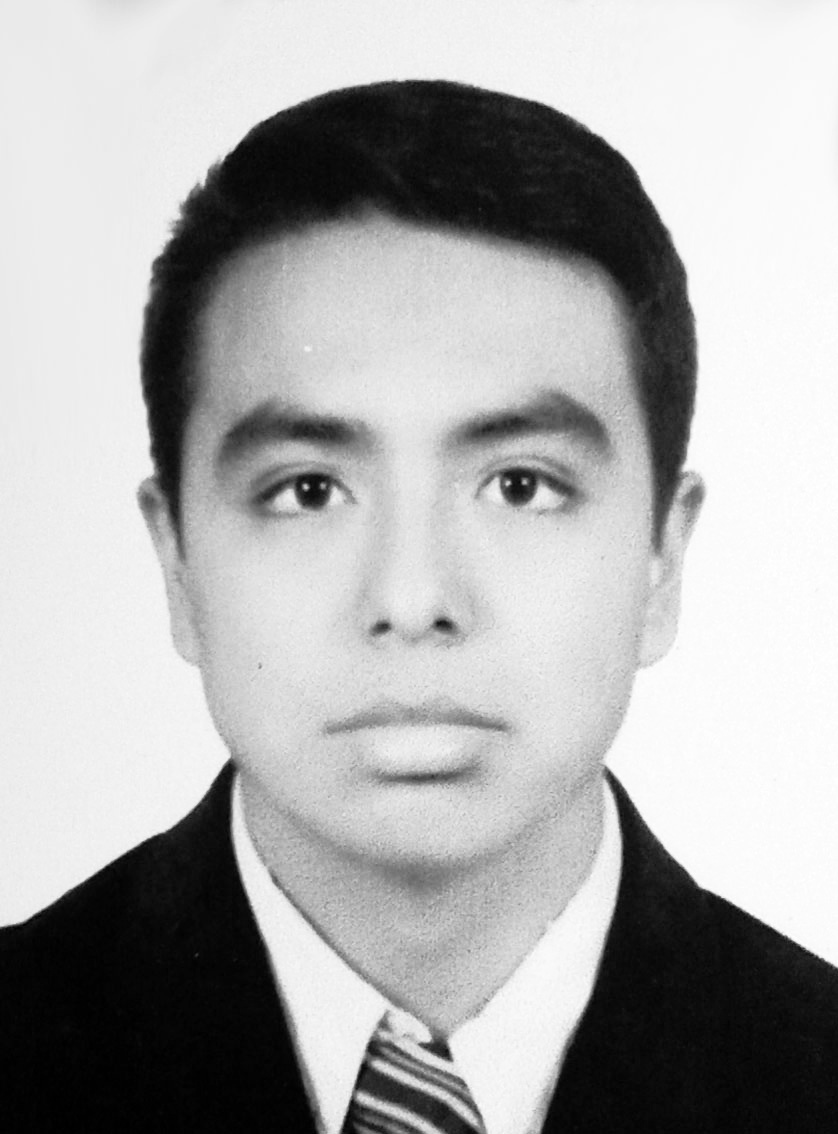
\includegraphics[width=1\columnwidth]{photo.jpg}\\[\baselineskip] % Your photo
\small % Smaller font size

\includegraphics[width=0.5cm,height=0.5cm]{icons/name.png}
Alexi  Uriel Cabrera Mayoral\\ % Your name

\includegraphics[width=0.5cm,height=0.5cm]{icons/email.png}
\url{alexi.cmayoral@gmail.com} \\ % Your email address

\includegraphics[width=0.5cm,height=0.5cm]{icons/phone.png}
55 8108 4753 \\ % Your phone number

\includegraphics[width=0.4cm,height=0.4cm]{icons/git.png}
\url{github.com/Kmabay}\\
\Sep % Some whitespace

\includegraphics[width=0.5cm,height=0.5cm]{icons/dir.png}
Alcatraz 15 \\ % Address 1
Sta. Rosa Chicoloapan \\
Edo. Méx. CP. 56370\\
\Sep

\includegraphics[width=0.5cm,height=0.5cm]{icons/languajes.png} English High-intermediate\\
\vfill % Whitespace under this block to push it up under the photo
\end{flushright}
}

%--------------------------------------------------------------------------------

\begin{document}
\userinformation % Print your information in the left column
\framebreak % End of the first column

%--------------------------------------------------------------------------------
%	HEADING
%--------------------------------------------------------------------------------

\cvheading{Alexi Cabrera} % Large heading - your name
%\cvsubheading{Engineering student} % Subheading - your occupation/specialization

%--------------------------------------------------------------------------------
%	ABOUT ME
%--------------------------------------------------------------------------------

\aboutme{Sobre mí}{Ingeniero en computación. Apasionado por la programación, matemáticas, NLP, UX/UI, \textit{data science} y bases de datos. Busco la oportunidad de contribuir a proyectos de vanguardia que involucren temas de mi interés e incrementar mis habilidades y conocimientos.}
%--------------------------------------------------------------------------------
%	EDUCATION
%--------------------------------------------------------------------------------
\CVSection{Educación}
\begin{tabular}{lllr}
    \textbf{FI UNAM}& \textit{Licenciatura} & Ing. en Computación & 2016 - 2024 (tentativo)\\
    \textbf{UnADM}& \textit{Licenciatura} & Matemáticas & 2017 - 2026 (tentativo)\\
    \textbf{UNAM}& \textit{Técnico} & Mantenimiento TI & 2014 - 2015\\
    \textbf{SEP}& \textit{Técnico} & Diseño gráfico & 2013 - 2014
\end{tabular}\Sep
%------------------------------------------------------------------------------
%	EXPERIENCE
%------------------------------------------------------------------------------
\CVSection{Experiencia}
\CVItem{Laboral}{
\begin{itemize}
    \item \textbf{HA Pedregal - Sistemas de información} \qquad\qquad 05/2023 - 02/2024\\
    {Configuré equipos de red y cómputo. Dí soporte y solución a incidentes y solicitudes de diferentes áreas del hospital y proveedores. Propusé soluciones durante la migración de sistema (S/4Hana). Me involucré en el desarrollo del cableado estructurado de una nueva torre hospitalaria.}\\
    \item \textbf{Centro académico Elyon - Docente} \qquad\qquad\qquad 02/2022 - 01/2023\\
    {Proporcioné enseñanza y apoyo en matemáticas, física e informática a personas de distintas edades y en distintos niveles de conocimiento.}\\
    \item \textbf{Instituto de Compuinglés de Oriente - Docente} \qquad\quad 07 - 10/2019\\
    {Practiqué la docencia en diseño gráfico y computación (Software de Microsoft y Adobe). Cumplí con las certificaciones requeridas por el instituto.}\\
    \item \textbf{Ingenia - Técnico} \qquad\qquad\qquad\qquad\qquad\qquad\qquad04/2014 - 04/2016\\
    {Realicé mantenimiento y reparación de equipos personales (PC's, laptops, tablets, celulares). Aprendí y realicé cotizaciones y venta de equipo de cómputo dependiendo las necesidades del cliente.}
\end{itemize}
}
%------------------------------------------------
\CVItem{Proyectos}{\begin{itemize}
    \item \textbf{Papiit-Papime y Conacyt - Desarrollador} \qquad\qquad\qquad\qquad 12/2022\\
    \textit{WebApp Paráfrasis}: Proyecto desarrollado en Flask, que calcula similitud semántica con diferentes algoritmos y LLM's.\\
    \item \textbf{Mozilla, UNAM - Miembro de Amoxcalli} \qquad\qquad\qquad\qquad 05/2022\\
    \textbit{Amoxcalli}: Biblioteca digital colaborativa de audio, con modelos pre-entrenados recolectamos datos del habla (español y lenguas indígenas de México). Primer lugar\textit{ Hackaton sobre tecnologías del habla}.\\
    \item \textbf{Papiit-Papime - Participante} \qquad\qquad\qquad\qquad\qquad\quad 02 - 08/2022\\
    \textit{PARMEX}: Involucrado en la implementación de herramientas de NLP y estudio de sus resultados.
\end{itemize}}
\Sep
%------------------------------------------------------------------------------
%	SKILLS
%\CVSection{Job skills} I work under pressure, Willingness to learn something needed soon
%------------------------------------------------------------------------------


\includegraphics[width=10cm,height=27cm]{space.png}

\CVSection{Habilidades y conocimientos}
\CVItem{Cursos y certificados}{
\begin{itemize}
    \item \textbf{SEP ICO Texcoco(2014):} Bases de datos con Microsoft Access
    \item \textbf{FI UNAM Proteco (2017):} Desarrollo web avanzado
    \item \textbf{FI UNAM Copadi (2018):} Métodos de demostración matemática
    \item \textbf{CISCO (2020):} PCAP (Programming Essentials in Python)
    \item \textbf{CISCO (2020):} Introducción a la ciberseguridad
    \item \textbf{freeCodeCamp (2021):} Python sk-learn Tutorial – ML Crash Course
    \item \textbf{CodeWarriors UDEMY (2021):} NLP Course for Beginner
    \item \textbf{SuperDataScience team UDEMY (2021):} Natural Language Processing (NLP) with BERT
    \item \textbf{Vinay Kummar UDEMY (2021):} Node, Express, React JS & MySQL full stack web development
    \item \textbf{Google Cloud Coursera (2022):} Google Cloud Fundamentals
\end{itemize}}
\Sep
\CVItem{Lenguajes y software de propósito general}{
\begin{itemize}
    \item Python: librerías NLP (Gensim, Spacy, scikit-learn, PyTorch, TensorFlow).
    \item Lenguajes enfocados a la ciencia de datos: Python (matplotlib), R.
    \item Programación en general: C, C++, Java.
\end{itemize}}
\Sep
\CVItem{Herramientas de infraestructura}{
\begin{itemize}
    \item Active Directory (UserAdmin y configuración de e-mail).
    \item Google cloud services (Contribución al deploy de una IA generativa basada en dark data, conocimiento básico de Looker Studio)
    \item SAP S/4Hana (ECH, Fiori, conocimiento básico de ABAP).
    \item Herramientas de Quality assurance (Agile, casos de uso, Postman, SQL).
    \item Linux, contenedores, Podman, Kubernetes
    \item Integración de microprocesadores (Raspberry Pi) y microcontroladores (Arduino), con protocolos de comunicación (UART, I2C, TCP/IP) y aplicaciones de ROS.
    \item Conocimiento de OpenGL a través de GLFW (shaders, primitivas, animación e iluminación).
    \item Uso de \LaTeX desde reportes académicos hasta tesis.
    \item Programación básica de micro PIC16F877 y Procesador MC88110.
\end{itemize}}
\Sep
\CVItem{Habilidades duras y blandas}{
\begin{itemize}
    \item Solución de problemas
    \item Habilidad analítica
    \item Ojo clínico 
    \item Comunicación y habilidades de trabajo en equipo
\end{itemize}}
\Sep
\CVItem{Temas abordados}{
\begin{itemize}
    \item Fundamentos de Deep learning
    \item Algoritmos de Machine learning
    \item Fundamentos de QA
    \item Principios de ingeniería de software
    \item Entendimiento de arquitecturas de CPU, GPU y FPGA
\end{itemize}}
\Sep

\end{document}
